% Theory for Project 01 — Your first HTTP API.
% Build (from this folder):  tectonic theory.tex   ->  theory.pdf
\documentclass[11pt,a4paper]{article}
\usepackage[T1]{fontenc}
\usepackage{lmodern}
\usepackage[margin=22mm]{geometry}
\usepackage{graphicx}
\usepackage{booktabs}
\usepackage{tabularx}
\usepackage{array}
\usepackage{enumitem}
\usepackage[table]{xcolor}
\usepackage{fancyvrb}
\usepackage{titlesec}
\usepackage[hidelinks]{hyperref}

\definecolor{accent}{HTML}{3367D6}
\definecolor{boxbg}{HTML}{F4F6FA}
\titleformat{\section}{\large\bfseries\color{accent}}{\thesection}{0.6em}{}
\titleformat{\subsection}{\normalsize\bfseries}{\thesubsection}{0.6em}{}
\setlength{\parindent}{0pt}
\setlength{\parskip}{0.55em}
\setlist{itemsep=0.15em, topsep=0.3em}
\renewcommand{\arraystretch}{1.25}
\newcolumntype{L}{>{\raggedright\arraybackslash}X}
\newcommand{\code}[1]{\texttt{#1}}

\newcommand{\keypoint}[1]{%
  \par\smallskip\noindent\colorbox{boxbg}{\parbox{\dimexpr\linewidth-2\fboxsep}{\small #1}}\par\smallskip}

\title{\textbf{Project 01 --- Your first HTTP API}\\[0.3em]\large Theory, answers and design decision}
\author{APIs: 24 Build-It-Yourself Projects}
\date{5 November 2026 \quad\textbullet\quad FastAPI 0.162.0, Starlette 1.10.0, Pydantic 2.14.2, uvicorn 0.54.0, Python 3.13.18}

\begin{document}
\maketitle

\keypoint{\textbf{How to read this.} Every claim about \emph{our} API was checked
against the running code (TestClient or a live uvicorn server, 2026-10-30 and
2026-11-05). Claims about HTTP itself cite RFC~9110 (HTTP Semantics). Where
something was measured rather than read, the text says so.}

\setcounter{tocdepth}{1}
\tableofcontents

% =====================================================================
\section{HTTP in five parts}

An HTTP exchange is one request and one response. RFC~9110 separates every
message into the same few parts. Our captured exchange shows all of them:

\begin{Verbatim}[fontsize=\small, frame=single, framesep=2mm]
> GET /hello?name=Nick HTTP/1.1          <- method + target + version
> Host: 127.0.0.1:8000                   <- headers (metadata)
> Accept: */*
>                                        <- empty line: headers end
< HTTP/1.1 200 OK                        <- status
< content-type: application/json         <- headers describing the body
< content-length: 27
< server-timing: app;dur=2.08
<
{"greeting":"Hello, Nick!"}              <- representation (the body)
\end{Verbatim}

\begin{tabularx}{\linewidth}{@{}l L L@{}}
\toprule
\textbf{Part} & \textbf{What it is} & \textbf{In our API} \\
\midrule
Method & What the client wants to do with the resource. \code{GET} means
``give me a representation''; it is \emph{safe} (no state change) and
\emph{idempotent} (repeating it changes nothing) (RFC~9110 \S9.2). &
Both routes are \code{GET} only. Anything else on a known path is \code{405}. \\
Target & The resource: a \emph{path} plus an optional \emph{query string}
after \code{?}. The router matches on the path only. &
\code{/hello} picks the handler; \code{name=Nick} becomes the function
argument \code{name}. \\
Headers & Name/value metadata about the message, not the content itself. &
\code{content-type} and \code{content-length} come from FastAPI;
\code{date} and \code{server} from uvicorn; \code{server-timing} from our
middleware. \\
Status & A three-digit code: 2xx success, 3xx redirect, 4xx client error,
5xx server error (RFC~9110 \S15). &
We return only 200, 404, 405 and 422, all on purpose (R05). \\
Representation & The body, plus the headers that say how to read it. &
Always JSON, declared by \code{content-type: application/json} (R03). \\
\bottomrule
\end{tabularx}

\subsection{Why the status code is not the whole story}
The status tells the client \emph{which kind} of outcome happened; the body
tells it \emph{the details}. A \code{200} with a wrong body is still a broken
API. That is why the tests check the status \emph{and} the exact JSON
(\code{response.json() == \{...\}}), not just the status.

% =====================================================================
\section{The layers a request passes through}

Our project is one file, but four libraries handle the request:

\begin{enumerate}
  \item \textbf{uvicorn} (an ASGI server) listens on a TCP port, reads bytes,
        turns them into a request, and later writes the response bytes. It adds
        \code{date} and \code{server}.
  \item \textbf{Starlette} (inside FastAPI) runs the middleware and the
        \emph{router}: it matches the path, then the method.
  \item \textbf{FastAPI} reads the function signature
        (\code{name: str = Query(...)}) and validates the query string
        \emph{before} calling our function.
  \item \textbf{Pydantic} does the actual validation, and turns the returned
        model into JSON through \code{response\_model}.
\end{enumerate}

Our own code is only the middleware \code{time\_and\_log} and the two handler
functions. Everything else is framework behavior, which is why we
\emph{measured} it instead of assuming it (Section~\ref{sec:measured}).

\begin{center}
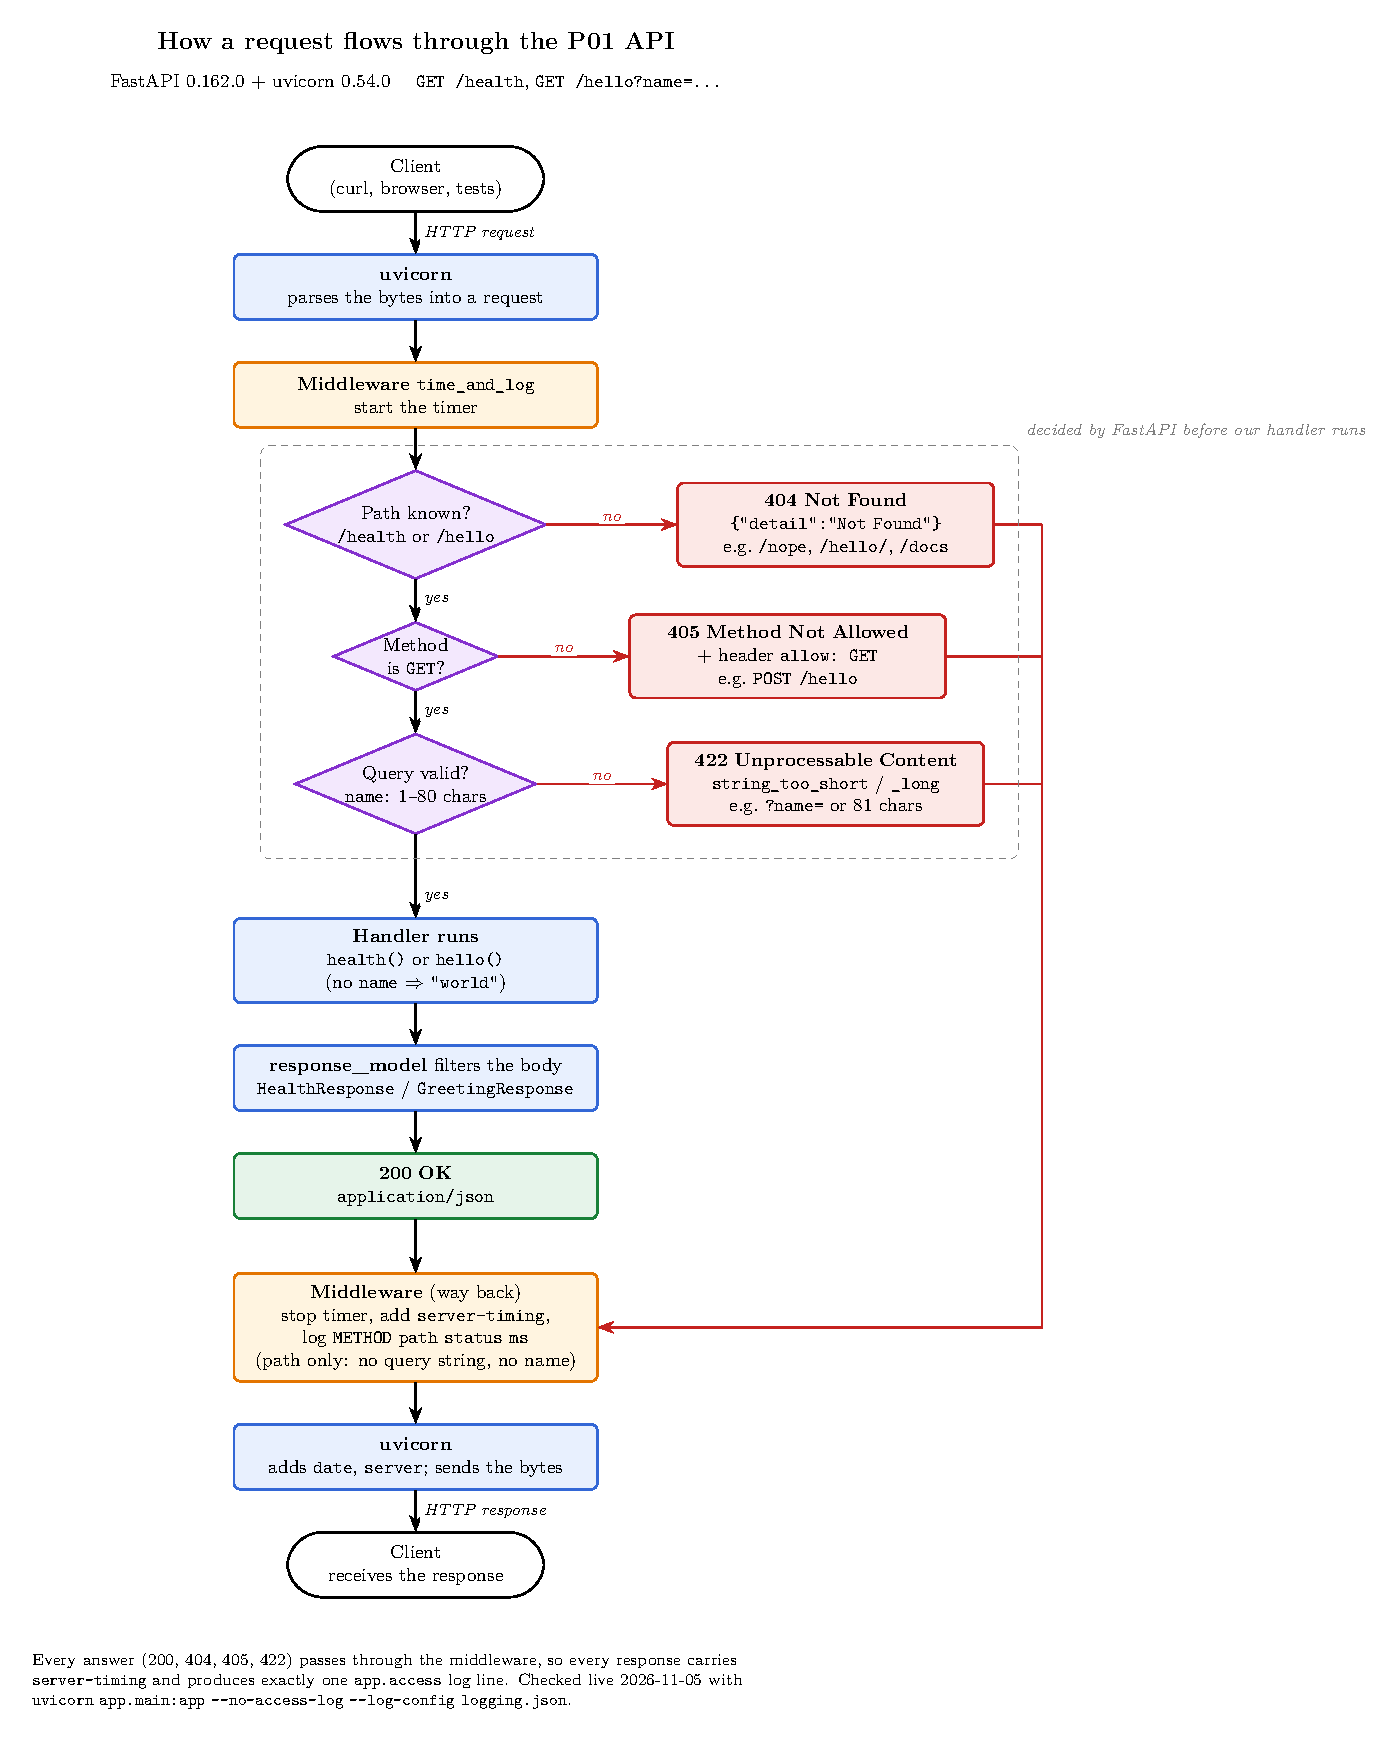
\includegraphics[height=0.74\textheight]{request-flow.pdf}
\end{center}

The order matters: \textbf{path, then method, then validation}. So
\code{POST /nope} is a 404 (the path fails first), \code{POST /hello} is a
405, and \code{GET /hello?name=} is a 422. The middleware wraps all of it, so
every outcome, including errors, is timed and logged.

% =====================================================================
\section{Status codes we return, and why}

\begin{tabularx}{\linewidth}{@{}l L L@{}}
\toprule
\textbf{Status} & \textbf{Meaning (RFC~9110)} & \textbf{When we send it} \\
\midrule
\code{200 OK} & The request succeeded; the body is the result (\S15.3.1). &
Valid \code{GET /health} or \code{GET /hello}. \\
\code{404 Not Found} & No current representation for the target (\S15.5.5). &
Any other path: \code{/nope}, \code{/HELLO}, \code{/hello/}, \code{/docs}. \\
\code{405 Method Not Allowed} & The target exists but does not support this
method. The server \textbf{MUST} send an \code{Allow} header listing the methods
it does support (\S15.5.6). &
\code{POST}, \code{PUT}, \code{DELETE}, \code{PATCH} on either route. We send
\code{allow: GET}. \\
\code{422 Unprocessable Content} & The request is well-formed, but its content
cannot be processed (\S15.5.21). The old name was ``Unprocessable Entity''. &
\code{name} is empty or longer than 80 characters (R04). \\
\bottomrule
\end{tabularx}

\subsection{The status we removed: 307}
By default FastAPI answers \code{GET /hello/} with \code{307 Temporary
Redirect} to \code{/hello}, with an empty body and no \code{content-type}.
That is a status we never chose, and a body that is not JSON. It breaks R03
and R05. Setting \code{redirect\_slashes=False} makes \code{/hello/} an
ordinary 404. This was our \textbf{independently discovered failure}: the test
went red (2 failed), and after the fix it went green (22/22).

\subsection{404 vs 422: which part of the request was wrong?}
404 and 405 are about the \emph{target and method}: the client asked for
something that does not exist. 422 is about the \emph{content}: the client
reached a real route but sent unacceptable data. Keeping them apart tells the
client what to fix.

% =====================================================================
\section{Validation at the boundary}

\code{Query("world", min\_length=1, max\_length=80)} is a \emph{contract at
the boundary}: bad input is rejected before it reaches our code. Inside
\code{hello()}, \code{name} is guaranteed to be a string of 1--80 characters.

\begin{itemize}
  \item \textbf{Default.} No \code{name} at all means \code{"world"} (T01).
        That is different from \code{?name=}, which is \emph{present but
        empty}, so it is rejected (422).
  \item \textbf{Characters, not bytes (measured).} \code{max\_length} counts
        Unicode characters. 80 emoji (320 bytes in UTF-8) are accepted;
        81 emoji are rejected. So R04 bounds characters. If the real concern
        were memory or log size, a byte limit would be needed as well.
  \item \textbf{The 422 body echoes the input (measured).} The error contains
        \code{"input": "aaa...a"}, the rejected value. That is harmless here,
        but if a field held a password or token, the error would send it
        back. Later projects should not echo sensitive fields.
\end{itemize}

% =====================================================================
\section{Response models: a stable contract (R02)}

A client is written against field \emph{names}. If \code{greeting} became
\code{message}, every client would break, even with a \code{200}.
\code{response\_model=GreetingResponse} pins the shape: undeclared fields are
dropped before sending. We measured this: a stray \code{db\_password} key
leaked without \code{response\_model} and was dropped with it. A test pins the
field names, so a rename now fails a test instead of breaking clients.

% =====================================================================
\section{A running process is not a ready service}

\code{GET /health} returning \code{\{"status":"ok"\}} proves only that the
process is up and can answer HTTP. It says nothing about dependencies,
because this project has none. In later projects (database, queues) there are
two different questions:

\begin{tabularx}{\linewidth}{@{}l L L@{}}
\toprule
& \textbf{Liveness} & \textbf{Readiness} \\
\midrule
Question & Is the process alive? & Can it do real work right now? \\
Checks & Nothing beyond answering. & Database reachable, migrations applied, \dots \\
If it fails & Restart the process. & Stop sending traffic; do not restart. \\
\bottomrule
\end{tabularx}

Our \code{/health} is a liveness check. T06 also makes sure it never exposes
the environment: with \code{DATABASE\_PASSWORD} set to a canary value, neither
the body nor the headers contain it.

% =====================================================================
\section{Observing every request without leaking data}

\begin{itemize}
  \item \textbf{Timing.} The middleware measures the time with
        \code{time.perf\_counter()} (a monotonic clock, safe for durations) and
        sends it in the \code{server-timing} header (a W3C standard that
        browser dev tools display).
  \item \textbf{One log line per request:}
        \code{app.access GET /hello 200 2.08ms}.\\
        It logs \code{request.url.path}, which leaves out the query string, so the
        caller's \code{name} never reaches the log.
  \item \textbf{Two flags are needed on the real server.} uvicorn's own access
        log prints the full query string, so it is switched off with
        \code{-{}-no-access-log}. Our \code{app.access} logger has no handler
        unless \code{-{}-log-config logging.json} gives it one; without that,
        the lines are silently dropped. Tests could not show this, because
        pytest captures log records itself.
\end{itemize}

% =====================================================================
\section{Edge cases measured on 2026-11-05}\label{sec:measured}

These were not in the spec. They were measured with FastAPI's TestClient
against the current code, to learn what the framework does.

{\small
\begin{tabularx}{\linewidth}{@{}l l L@{}}
\toprule
\textbf{Request} & \textbf{Result} & \textbf{What it teaches} \\
\midrule
\code{HEAD /health} & \textbf{405}, \code{allow: GET} &
RFC~9110 \S9.1 says general-purpose servers \textbf{MUST} support \code{GET}
and \code{HEAD}. FastAPI's \code{@app.get} does not add \code{HEAD}.
A real gap: noted for later, not fixed in P01. \\
\code{OPTIONS /hello} & 405, \code{allow: GET} & No CORS or OPTIONS handling; fine for this scope. \\
\code{?name=a\&name=b} & 200, \code{Hello, b!} & A repeated parameter: the last value wins, silently. \\
\code{?name=\%20} (a space) & 200, \code{Hello,\ \ !} & \code{min\_length=1} counts a space as a character. ``Non-empty'' is not ``meaningful''. \\
\code{?name=<script>} & 200, echoed & Safe as JSON (\code{application/json}), but dangerous if a client inserts it into HTML. \\
\code{/hello?NAME=Nick} & 200, \code{Hello, world!} & Parameter names are case-sensitive; an unknown one is ignored. \\
\code{/health?x=1} & 200 & Unknown query parameters are ignored, not rejected. \\
80 / 81 emoji & 200 / 422 & Length is counted in characters, not bytes. \\
\bottomrule
\end{tabularx}
}

% =====================================================================
\section{The four workbook questions}

\subsection*{1. What information and state cross the contract boundary?}
\textbf{In:} a method, a path, and for \code{/hello} one optional query
parameter \code{name} (1--80 characters). Other headers and parameters are
ignored. \textbf{Out:} a status (200/404/405/422), a JSON body with fixed
fields (\code{status} or \code{greeting}, or FastAPI's \code{detail}), and the
headers \code{content-type}, \code{content-length}, \code{server-timing}, and
\code{allow} on 405. \textbf{State:} none. The API stores nothing between
requests, so every request can be understood on its own. Environment
variables are deliberately \emph{not} part of the output (T06).

\subsection*{2. Which invariant would stay true if the framework changed?}
The \emph{HTTP contract}, not the code: \code{GET /hello} with no name returns
\code{\{"greeting": "Hello, world!"\}}; a name of 81 characters gives 422; an
unknown path gives 404 with a JSON body; a wrong method gives 405 with
\code{Allow}; \code{/health} never contains secrets. These are what
\code{tests/test\_api.py} checks through HTTP requests, so the same tests
would still judge a rewrite in Flask or Starlette. Only
\code{test\_every\_route\_declares\_a\_response\_model} inspects FastAPI
internals; it would have to be rewritten.

\subsection*{3. Which failure could a successful status hide?}
\begin{itemize}
  \item A \code{200} with the wrong body: a renamed field, or a leaked secret.
        Tests compare the full JSON, and T06 searches for a canary.
  \item A \code{200} from a redirect: an HTTP client follows the \code{307}
        silently and reports the final \code{200}. Our tests use
        \code{follow\_redirects=False} to see what the server really sent.
  \item A green test suite that skipped a test: an accidentally indented
        \code{def} became a nested function and pytest still said
        ``33 passed''. The test count must go up when a test is added.
  \item A \code{/health} that says \code{ok} while a dependency is down
        (liveness vs readiness, Section~6).
  \item A request that ``works'' but leaks the name into uvicorn's access log.
\end{itemize}

\subsection*{4. What must be measured rather than read in the docs?}
Everything in Section~\ref{sec:measured}, plus: the number of routes FastAPI
adds by default (6, not 2); the \code{307} on a trailing slash; whether the
log line actually reaches the console on a real server; whether the 422 body
echoes input; and \textbf{latency}. The \code{server-timing} values seen so
far (0.15--2.08~ms) are single samples. Real percentiles (p50/p95/max) come
from \code{scripts/measure.py} in Milestone~7 and go into EVIDENCE.md.
They are not estimated here.

% =====================================================================
\section{Design decision}

\textbf{Chosen: one FastAPI file} (\code{app/main.py}): two Pydantic response
models, one middleware, two handlers, run by uvicorn's development server.

\textbf{Alternative considered: a layered layout} (routers, a service layer,
dependency injection, separate settings), the structure of Project~04.

\begin{tabularx}{\linewidth}{@{}l L L@{}}
\toprule
& \textbf{One file (chosen)} & \textbf{Layered} \\
\midrule
Meets R01--R06 & Yes (34 tests pass) & Yes, with more code \\
Request path & Readable top to bottom in one file & Spread across modules \\
Testability & Whole app via TestClient & Same, plus unit tests per layer \\
Cost now & 82 lines, comments included & Several files for two routes with no logic \\
Pays off when & Little logic, no state & Real business logic, storage, many routes \\
\bottomrule
\end{tabularx}

\textbf{Why one file meets this brief.} The workbook says: \emph{do not add
service layers before you can explain the request path}. With two routes and
no state, a service layer would hold nothing. FastAPI was chosen over plain
Starlette or \code{http.server} because it gives validation (R04), JSON
media type (R03), response filtering (R02) and correct 404/405 handling
(R05) without hand-written code.

\textbf{What it costs.} We depend on framework defaults, and some of them were
wrong for us (docs routes, slash redirects, no \code{HEAD}). Each one needed a
measurement and a test. The development server is single-process: fine for
learning, not a production deployment.

\textbf{What would make me change it.} A third route with real logic, any
storage, or settings that differ between environments. Then routers and a
service layer become worth their cost (Project~04).

% =====================================================================
\section{Cost}

Nothing billable was run: the API ran only on this laptop. The workbook's
worksheet assumes 1 instance $\times$ 4 hours $\times$ \$0.06 = \$0.24 per
practice period. That is a \emph{hypothetical rate}, not a measured invoice.
The only measured resources are local: the requests and their
\code{server-timing} durations.

% =====================================================================
\section{Reading}
\begin{itemize}
  \item RFC~9110, \emph{HTTP Semantics}:
        \S9 (methods), \S15 (status codes), \S8.3 (Content-Type).
        \url{https://www.rfc-editor.org/rfc/rfc9110.html}
  \item FastAPI tutorial: query parameters and string validation; response
        model. \url{https://fastapi.tiangolo.com/tutorial/}
  \item W3C, \emph{Server Timing}. \url{https://www.w3.org/TR/server-timing/}
\end{itemize}

\end{document}
